\documentclass[11pt, draft]{article}
\usepackage{lipsum,mathptmx,etoolbox}
\usepackage[american]{babel}
\usepackage[backend=biber, maxbibnames=100, style=ieee]{biblatex}
\renewcommand{\rmdefault}{phv} % Arial
\renewcommand{\sfdefault}{phv}
\usepackage{pgfgantt}
\usepackage{amsmath,amssymb}
\usepackage{xcolor}
\usepackage{booktabs}
\usepackage{pifont}
\usepackage[font={small}]{caption}
\usepackage{float}
\usepackage{xcolor}
\newcommand{\cmark}{\textcolor{green!60!black}{\ding{51}}}
\newcommand{\xmark}{\textcolor{red}{\ding{55}}}
\usepackage{tabularx}
\newcolumntype{Y}{>{\centering\arraybackslash}X}
\usepackage{csquotes}
\addbibresource{proposal.bib}
\usepackage{titlesec}
\titlespacing*\section{0pt}{-0pt plus 4pt minus 2pt}{0pt plus 2pt minus 2pt}
\titlespacing*\subsection{0pt}{-0pt plus 4pt minus 2pt}{0pt plus 2pt minus 2pt}
\titlespacing*\subsubsection{0pt}{-0pt plus 4pt minus 2pt}{0pt plus 2pt minus 2pt}

\setlength{\parindent}{.5cm}
\setlength{\parskip}{1.25ex}
\usepackage[
top    = 1.87cm,
bottom = 1.87cm,
left   = 1.27cm,
right  = 1.27cm]{geometry}
\usepackage{fancyhdr}
\pagestyle{fancy}
\renewcommand{\headrulewidth}{0pt}
\renewcommand{\footrulewidth}{0pt}
\lhead{}
\rhead{Talon Chandler}
\cfoot{}
\rfoot{\thepage}
\hyphenpenalty=1000
\begin{document}
\section*{Specific Aims}
Fluorescence microscopy is an extremely valuable tool in
biology---by introducing a fluorescent probe into a live organism and measuring
the position of the probe, researchers can watch cellular processes as they
occur. An extraordinary amount of effort has been expended towards improving the
spatial resolution of fluorescence microscopes, and recent breakthroughs have
allowed microscopes to achieve resolutions below the diffraction limit which has
enabled new biological insights \cite{nobel}.

Position is not the only property of fluorophores that can report on biological
processes, though. Early studies have shown that the \textit{orientation} of
fluorophores can report valuable information as well
\cite{weiss1999}. Unfortunately, current live-cell techniques can only measure
the transverse orientation of fluorophores in relatively thin specimens. These
constraints severely limit the number of biological questions that can be
answered using available orientation measurement techniques. In this work we
propose the use of polarized multiview microscopes to measure the
three-dimensional orientation of fluorophores in thick living specimens. We
believe that this class of techniques will enable new insights in structural and
functional biology.

\noindent\textbf{Hypothesis:} Three-dimensional fluorescence orientation microscopy is a
valuable tool for investigating structural and functional biology in living
cells.

\noindent\textbf{Aim 1:} Develop a signal processing pipeline for analyzing and visualizing polarized multiview fluorescence microscopy data.

The raw data collected by polarized multiview fluorescence microscopes is not
easily interpreted in terms of fluorophore orientations. We propose a signal
processing pipeline that can efficiently reconstruct fluorophore orientations
from polarized multiview fluorescence microscopy data. An essential piece of
this pipeline is the spherical Fourier transform---by analyzing the data in the
angular frequency domain we can reconstruct fluorescence orientations much more
efficiently that existing techniques.

\noindent\textbf{Aim 2:} Demonstrate and verify three-dimensional fluorescence
orientation microscopy using a dual-view light-sheet microscope and a
light-field microscope.

We propose two complementary three-dimensional fluorescence orientation
microscopes---a dual-view light-sheet microscope and a light-field
microscope. The dual-view light-sheet microscope has isotropic spatial
resolution and a large field of view, but it suffers from long imaging times and
it delivers a large light dose to the sample. The light-sheet microscope has
complementary strengths and weaknesses---it images quickly and delivers a small
light dose, but it suffers from anisotropic spatial resolution and has a
relatively small field of view.

\noindent\textbf{Aim 3:} Demonstrate the value of three-dimensional fluorescence orientation
microscopy for live-cell biology.

Our overarching goal is to develop useful tools that will enable biological
discovery. To achieve this goal we will work directly with biologists who will
propose specific questions and experiments for the techniques we are
proposing. We expect that these interactions will inform and redirect our work
in ways that will improve the likelihood of biological discovery.

\pagebreak

\section*{Research Strategy}
\subsection*{Background}
A \textit{fluorescence microscope} is an optical imaging system that can measure
the position of fluorescent objects with a resolution of 1 $\mu$m or better.
Fluorescence microscopes excite fluorophores in a sample using short-wavelength
light and detect the long-wavelength light that the fluorophores emit as they
relax. By focusing the emitted light onto a plane detector using a series of
lenses, a fluorescence microscope creates a two-dimensional image of the
fluorophores in a sample.

Fluorescence microscopes image fluorescent samples, so how can we attain a
fluorescent sample? \textit{(1)~Find fluorescent samples in nature.} Most
organisms create fluorescent molecules naturally. Chlorophyll, collagen, and
melanin are examples of fluorescent molecules that are found in many plants and
animals. \textit{(2)~Add a fluorescent dye to a sample.}  There are hundreds of
commercially-available fluorescent dyes that can be introduced into a
sample. Researchers can choose a dye that will bind to a structure or process
that they are interested in studying.\hspace{0.4em}\textit{(3)~Genetically
  modify an organism so that it creates fluorescent proteins.} Many organisms
can be genetically modified so that a specific protein of interest displays
fluorescence. These techniques can be used to image almost any biological
process that involves proteins.

Most fluorescence microscopes only measure the position of fluorescent objects,
but by adding \textit{polarizing filters} to the microscope we can also measure
the orientation of the fluorescent objects. If we place a polarizing filter in
the excitation light path, then the light that is incident on the sample is
polarized and it selectively excites fluorophores that are parallel to the
light's polarization. If we place a polarizing filter in the detection path,
then we only detect light of a specific polarization so we selectively detect
fluorophores that are parallel to the detected polarization. By collecting
images under several polarizing filter orientations and applying a
reconstruction scheme, we can find the position and orientation of fluorophores
in a sample.

\subsection*{Innovation}
Table 1 summarizes state-of-the-art techniques for measuring the orientation of
fluorophores. In this section we will briefly describe each technique and its
strengths and weaknesses. 

Polarized single-view microscopy \cite{demay2011} is the simplest fluorescence
orientation measurement technique. A simple single-view fluorescence microscope
can be modified into a polarized single-view microscope by adding a
liquid-crystal polarizing filter to the illumination or detection path. After
collecting intensity images under several polarizing filter orientations, the
orientation of fluorophores can be reconstructed by applying simple image
arithmetic to the set of images. Polarized single-view microscopes image quickly
and gently---many live-cell biology applications already use these
techniques---but they suffer from incomplete axial spatial and axial angular
resolution.

Single-molecule localization techniques do not require any special imaging
hardware---a plain fluorescence microscope can be used. Instead of special
hardware, a photo-activatable fluorophore is used so that the concentration of
excited fluorophores can be precisely controlled. By exciting and imaging
fluorophores one a time instead of all at once, the location and orientation of
the fluorophores can be determined extremely precisely. Although these techniques
can measure the position and orientation of fluorophores more precisely than any
other light-microscopy technique, they require extremely long imaging times and
large light doses. These constraints make localization techniques unsuitable for
many applications in biology where fast and gentle imaging are essential for
imaging live cells.

\begin{table}[t]
  \centering
  \begin{tabularx}{1\textwidth}{r *{4}{Y}}
    \toprule
&\multicolumn{2}{c}{Existing} &\multicolumn{2}{c}{Proposed} \\
\cmidrule(r){2-3} \cmidrule(r){4-5}
  & & Single- & Polarized &   \\
  Microscopy technique& Polarized single-view & molecule localization & dual-view light-sheet & Polarized light-field \\
  \midrule
Transverse spatial resolution & \cmark & \cmark\cmark\cmark & \cmark\cmark & \cmark \\
Axial spatial resolution & \xmark & \cmark\cmark\cmark & \cmark\cmark & \cmark \\
Transverse angular resolution & \cmark & \cmark & \cmark & \cmark \\
Axial angular resolution & \xmark & \cmark & \cmark & \cmark \\
Temporal resolution & \cmark & \xmark & \cmark & \cmark\cmark \\
Low dose & \cmark\cmark & \xmark & \cmark & \cmark\cmark \\
Inexpensive & \cmark\cmark & \cmark\cmark & \cmark & \cmark\cmark \\
Large field of view & \cmark & \cmark & \cmark\cmark & \cmark \\
\bottomrule
\end{tabularx}
  \caption{Comparison of existing and proposed fluorescence orientation microscopy techniques.}
\end{table}

Figure 1 shows the imaging geometry for the proposed polarized dual-view
light-sheet microscope. This technique uses two objectives instead of one, and
it selectively excites planes of the sample to reduce phototoxicity. By using
the images from both views, this technique can achieve isotropic spatial
resolution, and it can measure the three-dimensional orientation of fluorophores
throughout a large field of view. Although this technique does not achieve the
high spatial resolution of single-molecule localization techniques, it can be
applied to large-volume live-cell imaging.

Figure 2 shows an image collected by a light-field microscope. By replacing the
usual detector plane with a microlens array and moving the detector to the focal
plane of the microlenses, a light-field microscope captures many angular views
of the sample at once. We can use these views and limited-angle tomography
reconstruction techniques to determine the three-dimensional position of
fluorophores throughout a sample. We propose the addition of polarizing filters
to the light-field microscope to measure the three-dimensional orientation and
position of the fluorophores. While the proposed light-field approach has poorer
resolution than the dual-view light-sheet approach, the light-field approach is
extremely fast and gentle, and it will allow us to study fast-moving processes
for long periods.

\begin{figure}[t]
\centering
\begin{minipage}{.45\textwidth}
  \centering
  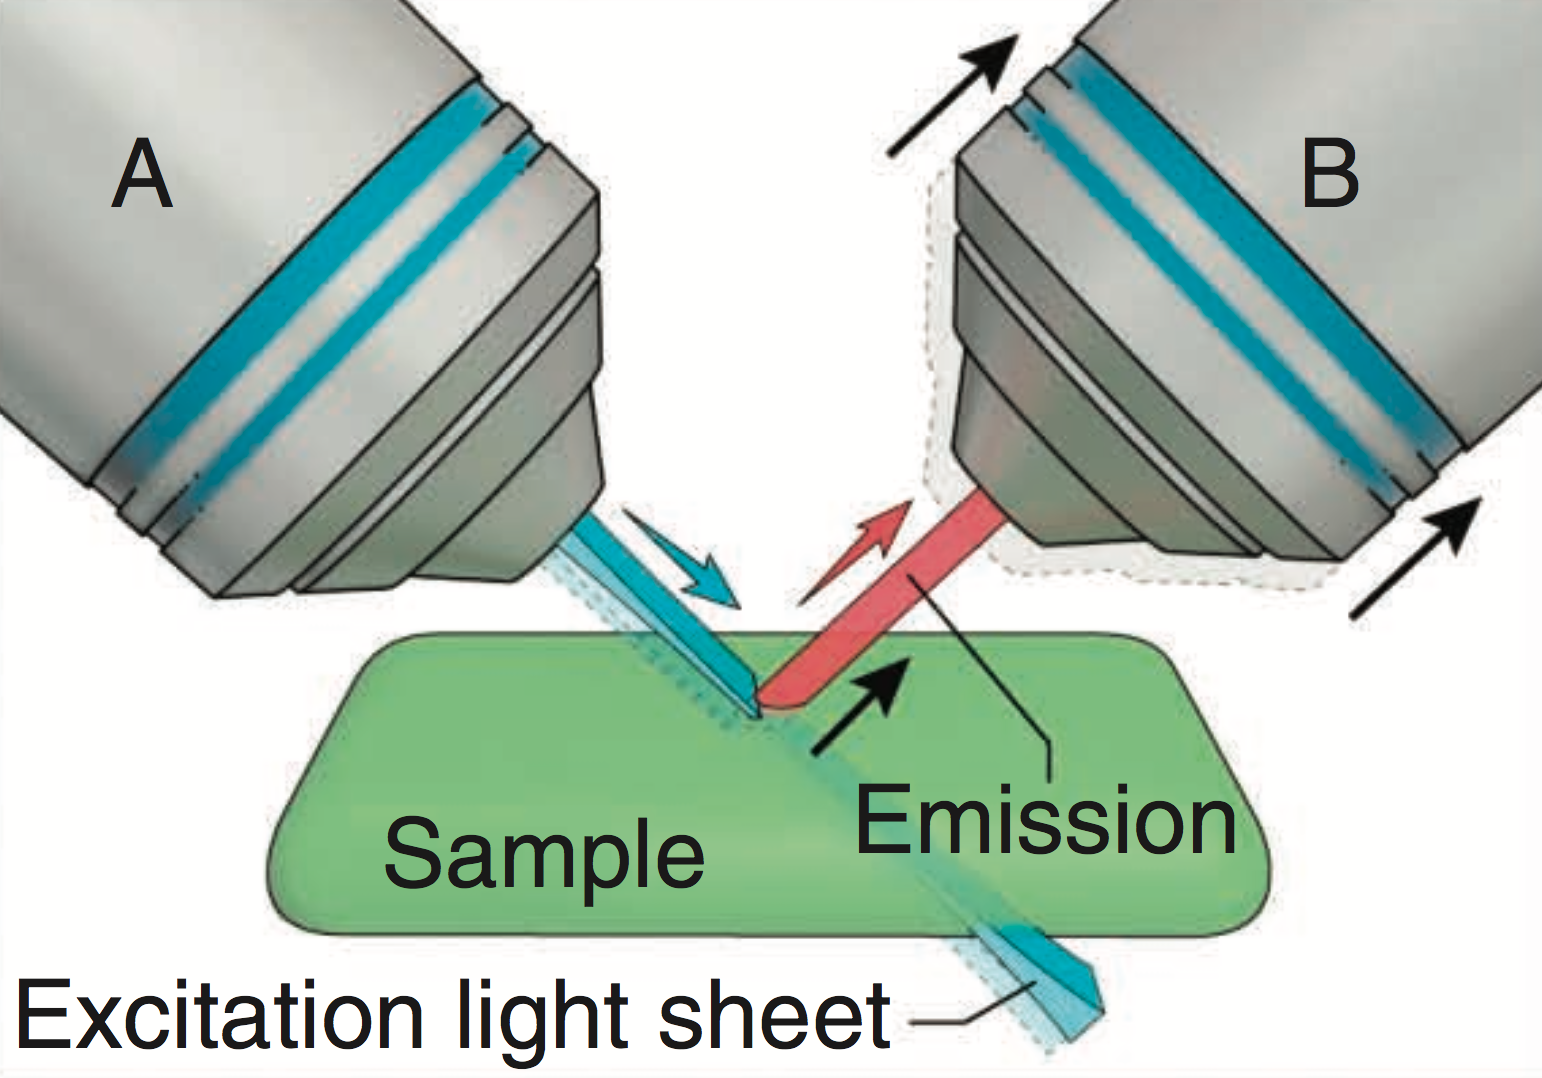
\includegraphics[width=\textwidth, interpolate=true]{figs/light-sheet}
  \caption{A dual-view light-sheet microscope excites the fluorophores in the
    sample with a light sheet originating from one objective, and it images the
    emitted light using the other objective as the light sheet sweeps through
    the sample. Next, the roles of the objectives are reversed and another set
    of images is acquired from the opposite view. We propose a dual-view
    light-sheet microscope outfitted with polarizing filters on each illumination
    arm. Figure from \cite{wu2013}.}
  \label{fig:test1}
\end{minipage}%
\hspace{0.75em}
\begin{minipage}{.45\textwidth}
  \centering
  \vspace{.96em}
  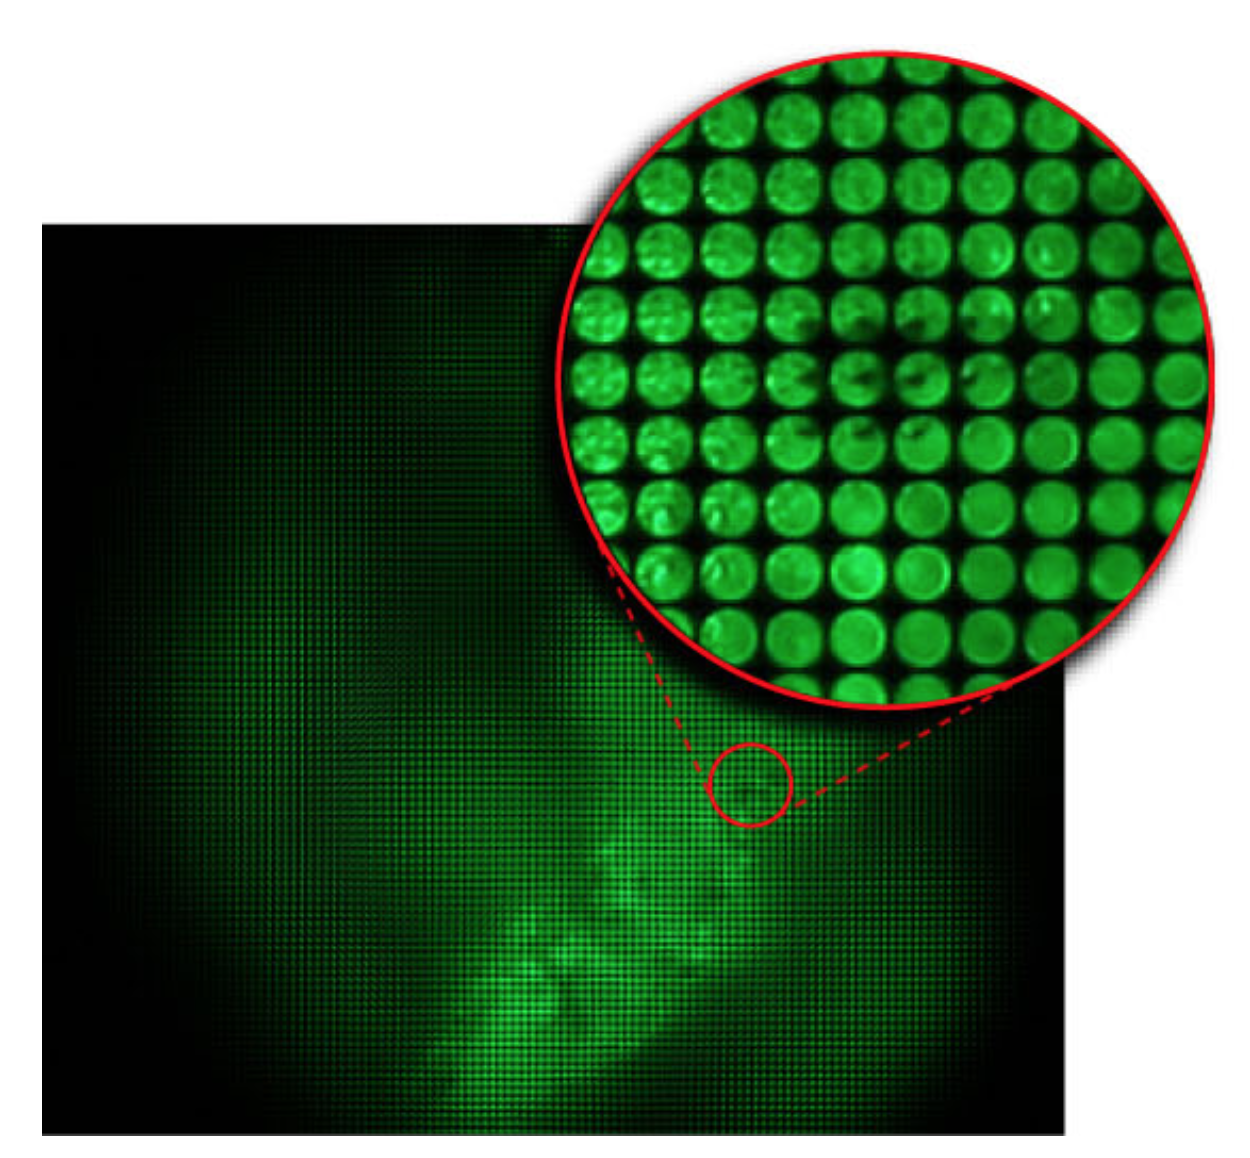
\includegraphics[width=\textwidth, interpolate=true]{figs/lf-fluo}
  \caption{A light-sheet microscope is an ordinary single-view microscope with a
    microlens array in the usual detector plane and the detector displaced to
    the focal plane of the microlenses. The image collected by a light-field
    microscope consists of many angular views of the sample collected at
    once. Figure from \cite{levoy2006}.}
  \label{fig:test2}
\end{minipage}
\end{figure}

\subsection*{Preliminary Results}
We have completed a theoretical study that investigates the limits of
orientation microscopy and the advantages of using multiple views
\cite{chandler17}. In addition to finding that multiview microscopes can measure
the orientation of fluorophores in all orientations instead of just transverse
orientations, we also developed a set of practical design heuristics that we
will apply to the design of our microscopes.

We have also collected preliminary data of a stained and fixed cell with a
polarized dual-view light-sheet microscope. Figure 3 shows a prototype
three-dimensional orientation reconstruction using a simplified model applied to
real data, and the results match our expectations.

Finally, we have collected preliminary images of several test specimens with
known fluorophore position and orientation including oriented fluorescent fibers
and giant unilamellar vesicles. These test specimens will be essential tools to
help us verify the results of our reconstructions.

\begin{figure}[t]
\centering
  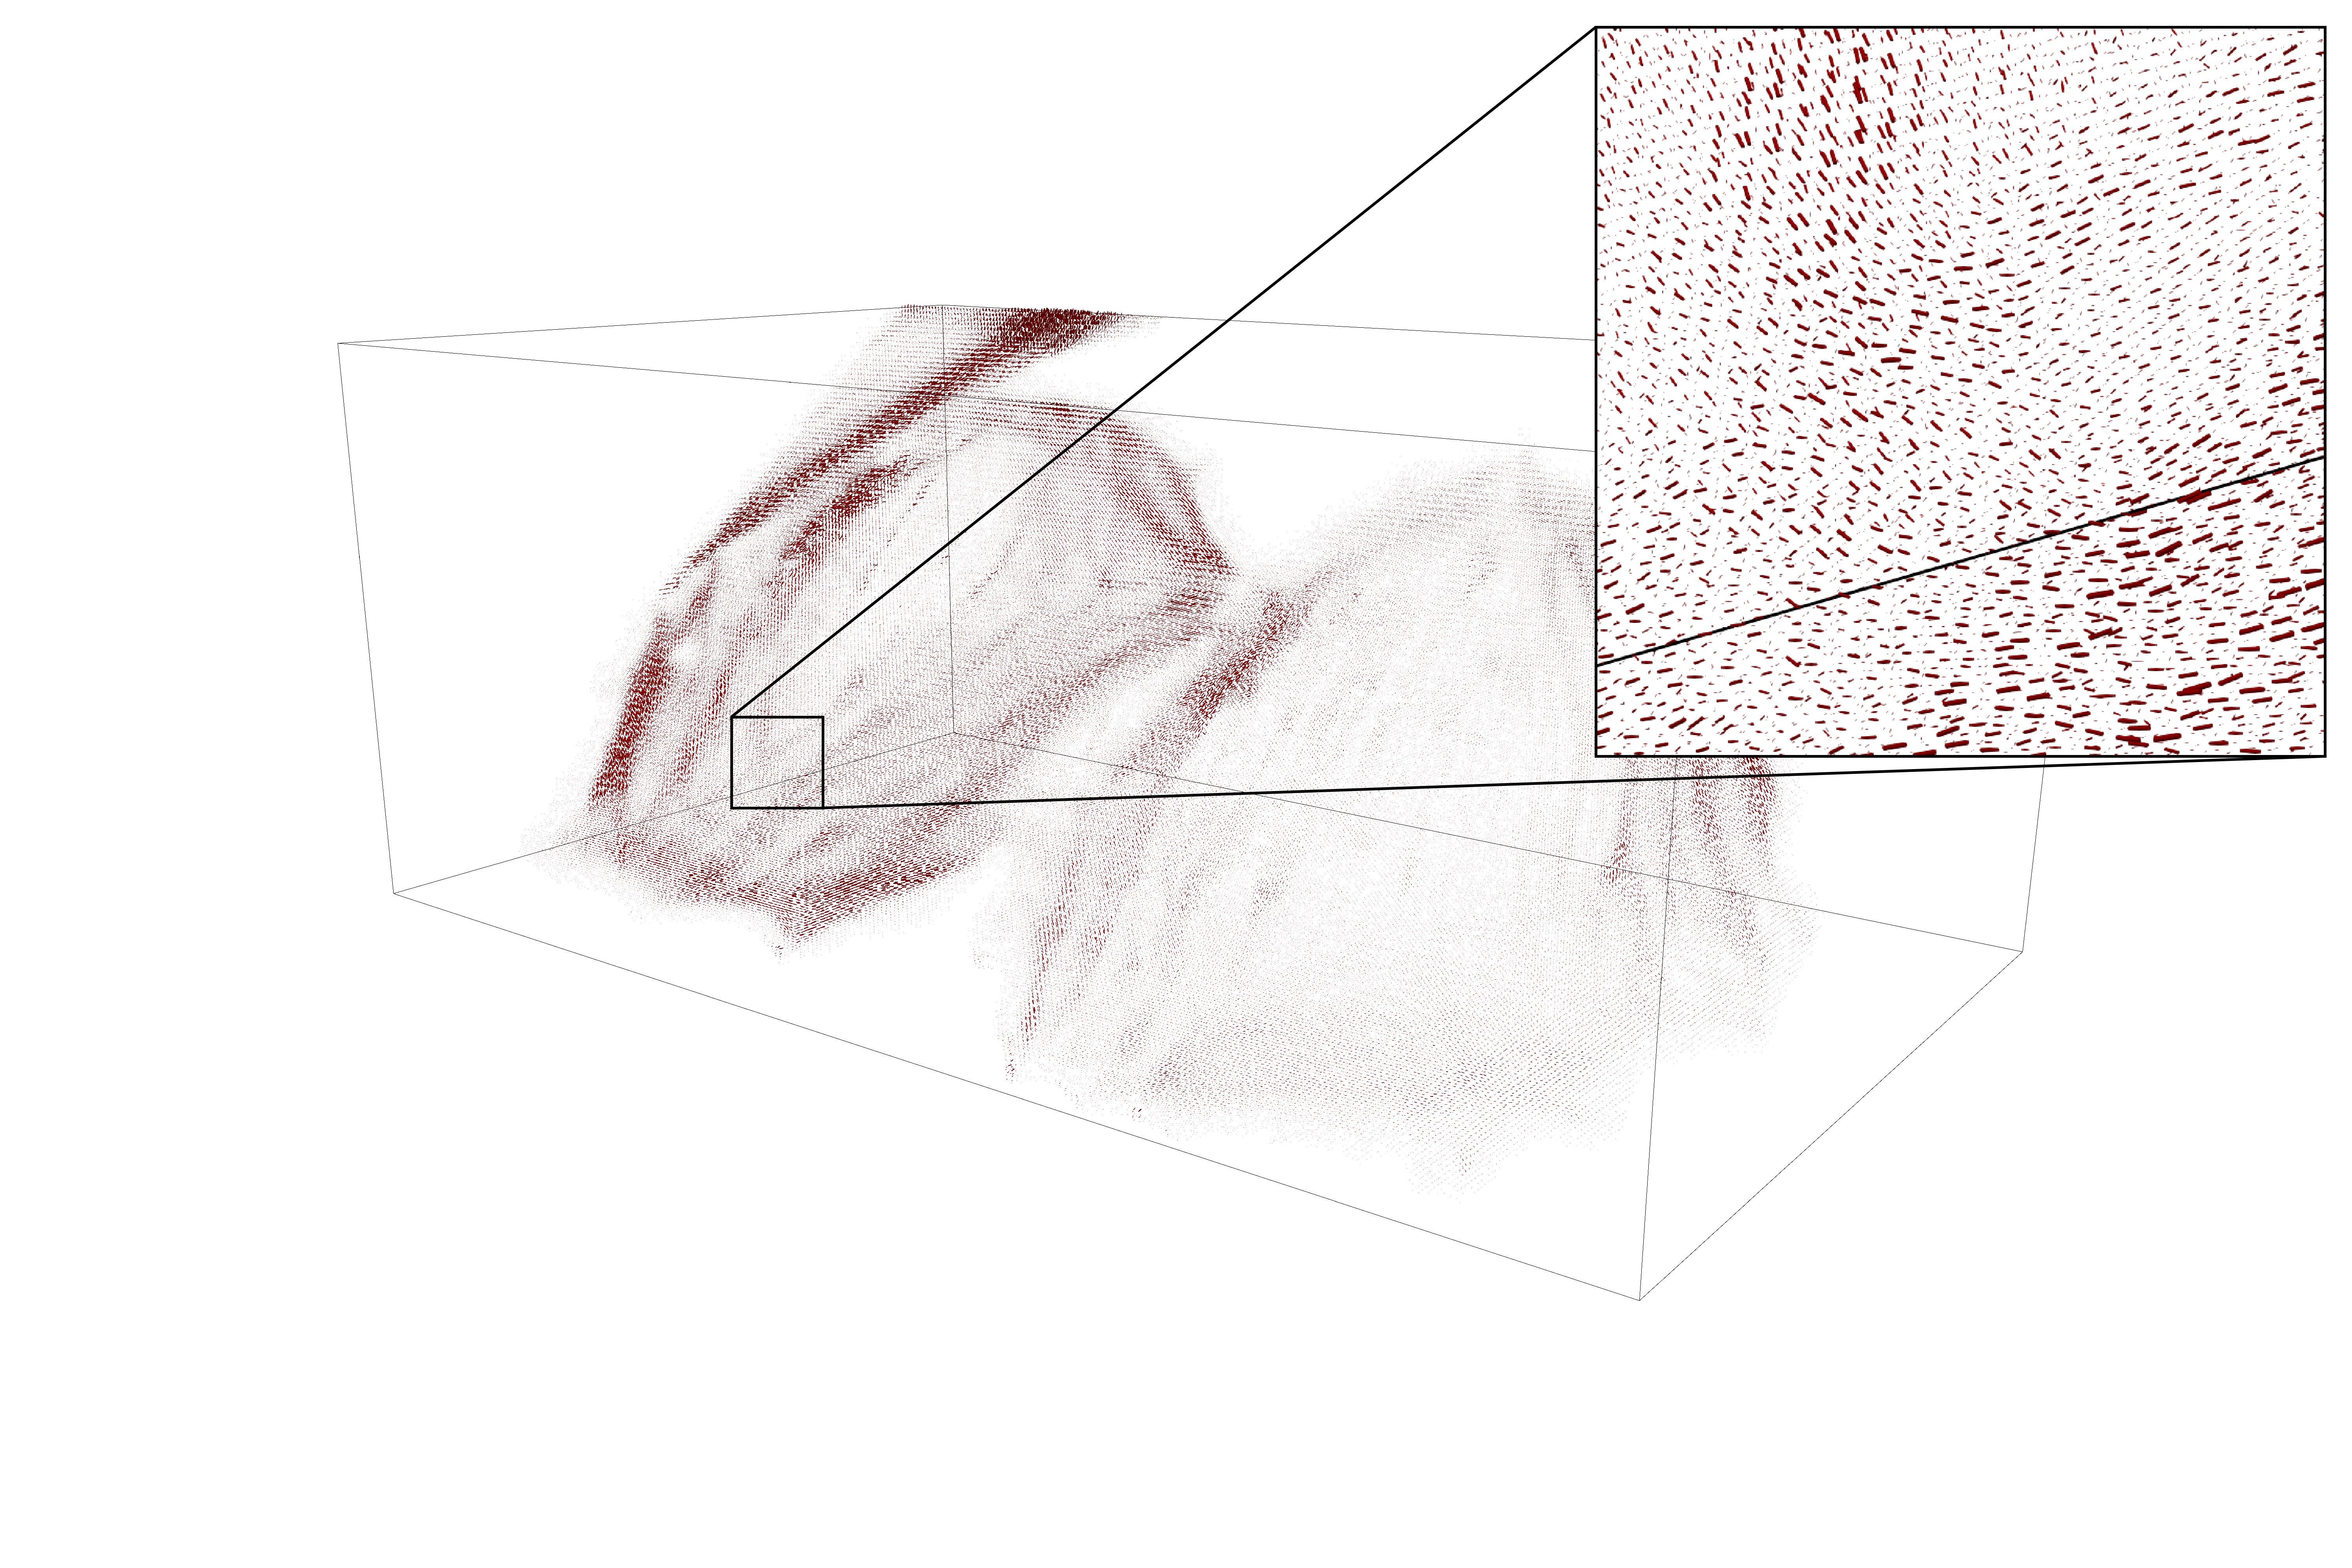
\includegraphics[width=0.65\textwidth, interpolate=true, trim={6em 4em 2em 0em}]{figs/inset}
  \caption{Orientation reconstruction of a 68$\times$108$\times$46 $\mu$m${}^3$
    volume of fixed cells stained with Alexa Fluor 488 Phalloidin and imaged
    with an asymmetric 1.1/0.71 NA dual-view light-sheet microscope. We assign a
    scaled and oriented glyph to each voxel to indicate the quantity and
    orientation of fluorophores in that voxel.}
  \label{fig:test1}
\end{figure}


\subsection*{Approach}
\noindent\textbf{Aim 1:} Develop a signal processing pipeline for analyzing and
  visualizing polarized multiview fluorescence microscopy data.

  \noindent\textbf{Methods:} We will use physical modeling, linear systems
  theory, and optimization techniques to develop an efficient signal processing
  pipeline for the proposed microscopes. We have completed a prototype signal
  processing pipeline for reconstructing the three-dimensional orientation of
  fluorophores from polarized dual-view light-sheet microscope data, and we plan
  to improve this work by relaxing our assumptions and extending it to the
  light-field microscope.

  We have also introduced the spherical Fourier transform for analyzing
  fluorescence orientation microscopes in the angular frequency domain---see
  Figures 4 and 5. These techniques allow us to use linear systems theory to
  understand our imaging systems, and we have already made large efficiency
  improvements by analyzing our microscopes in this way.
  
\begin{figure}
\centering
\begin{minipage}{.45\textwidth}
  \centering
  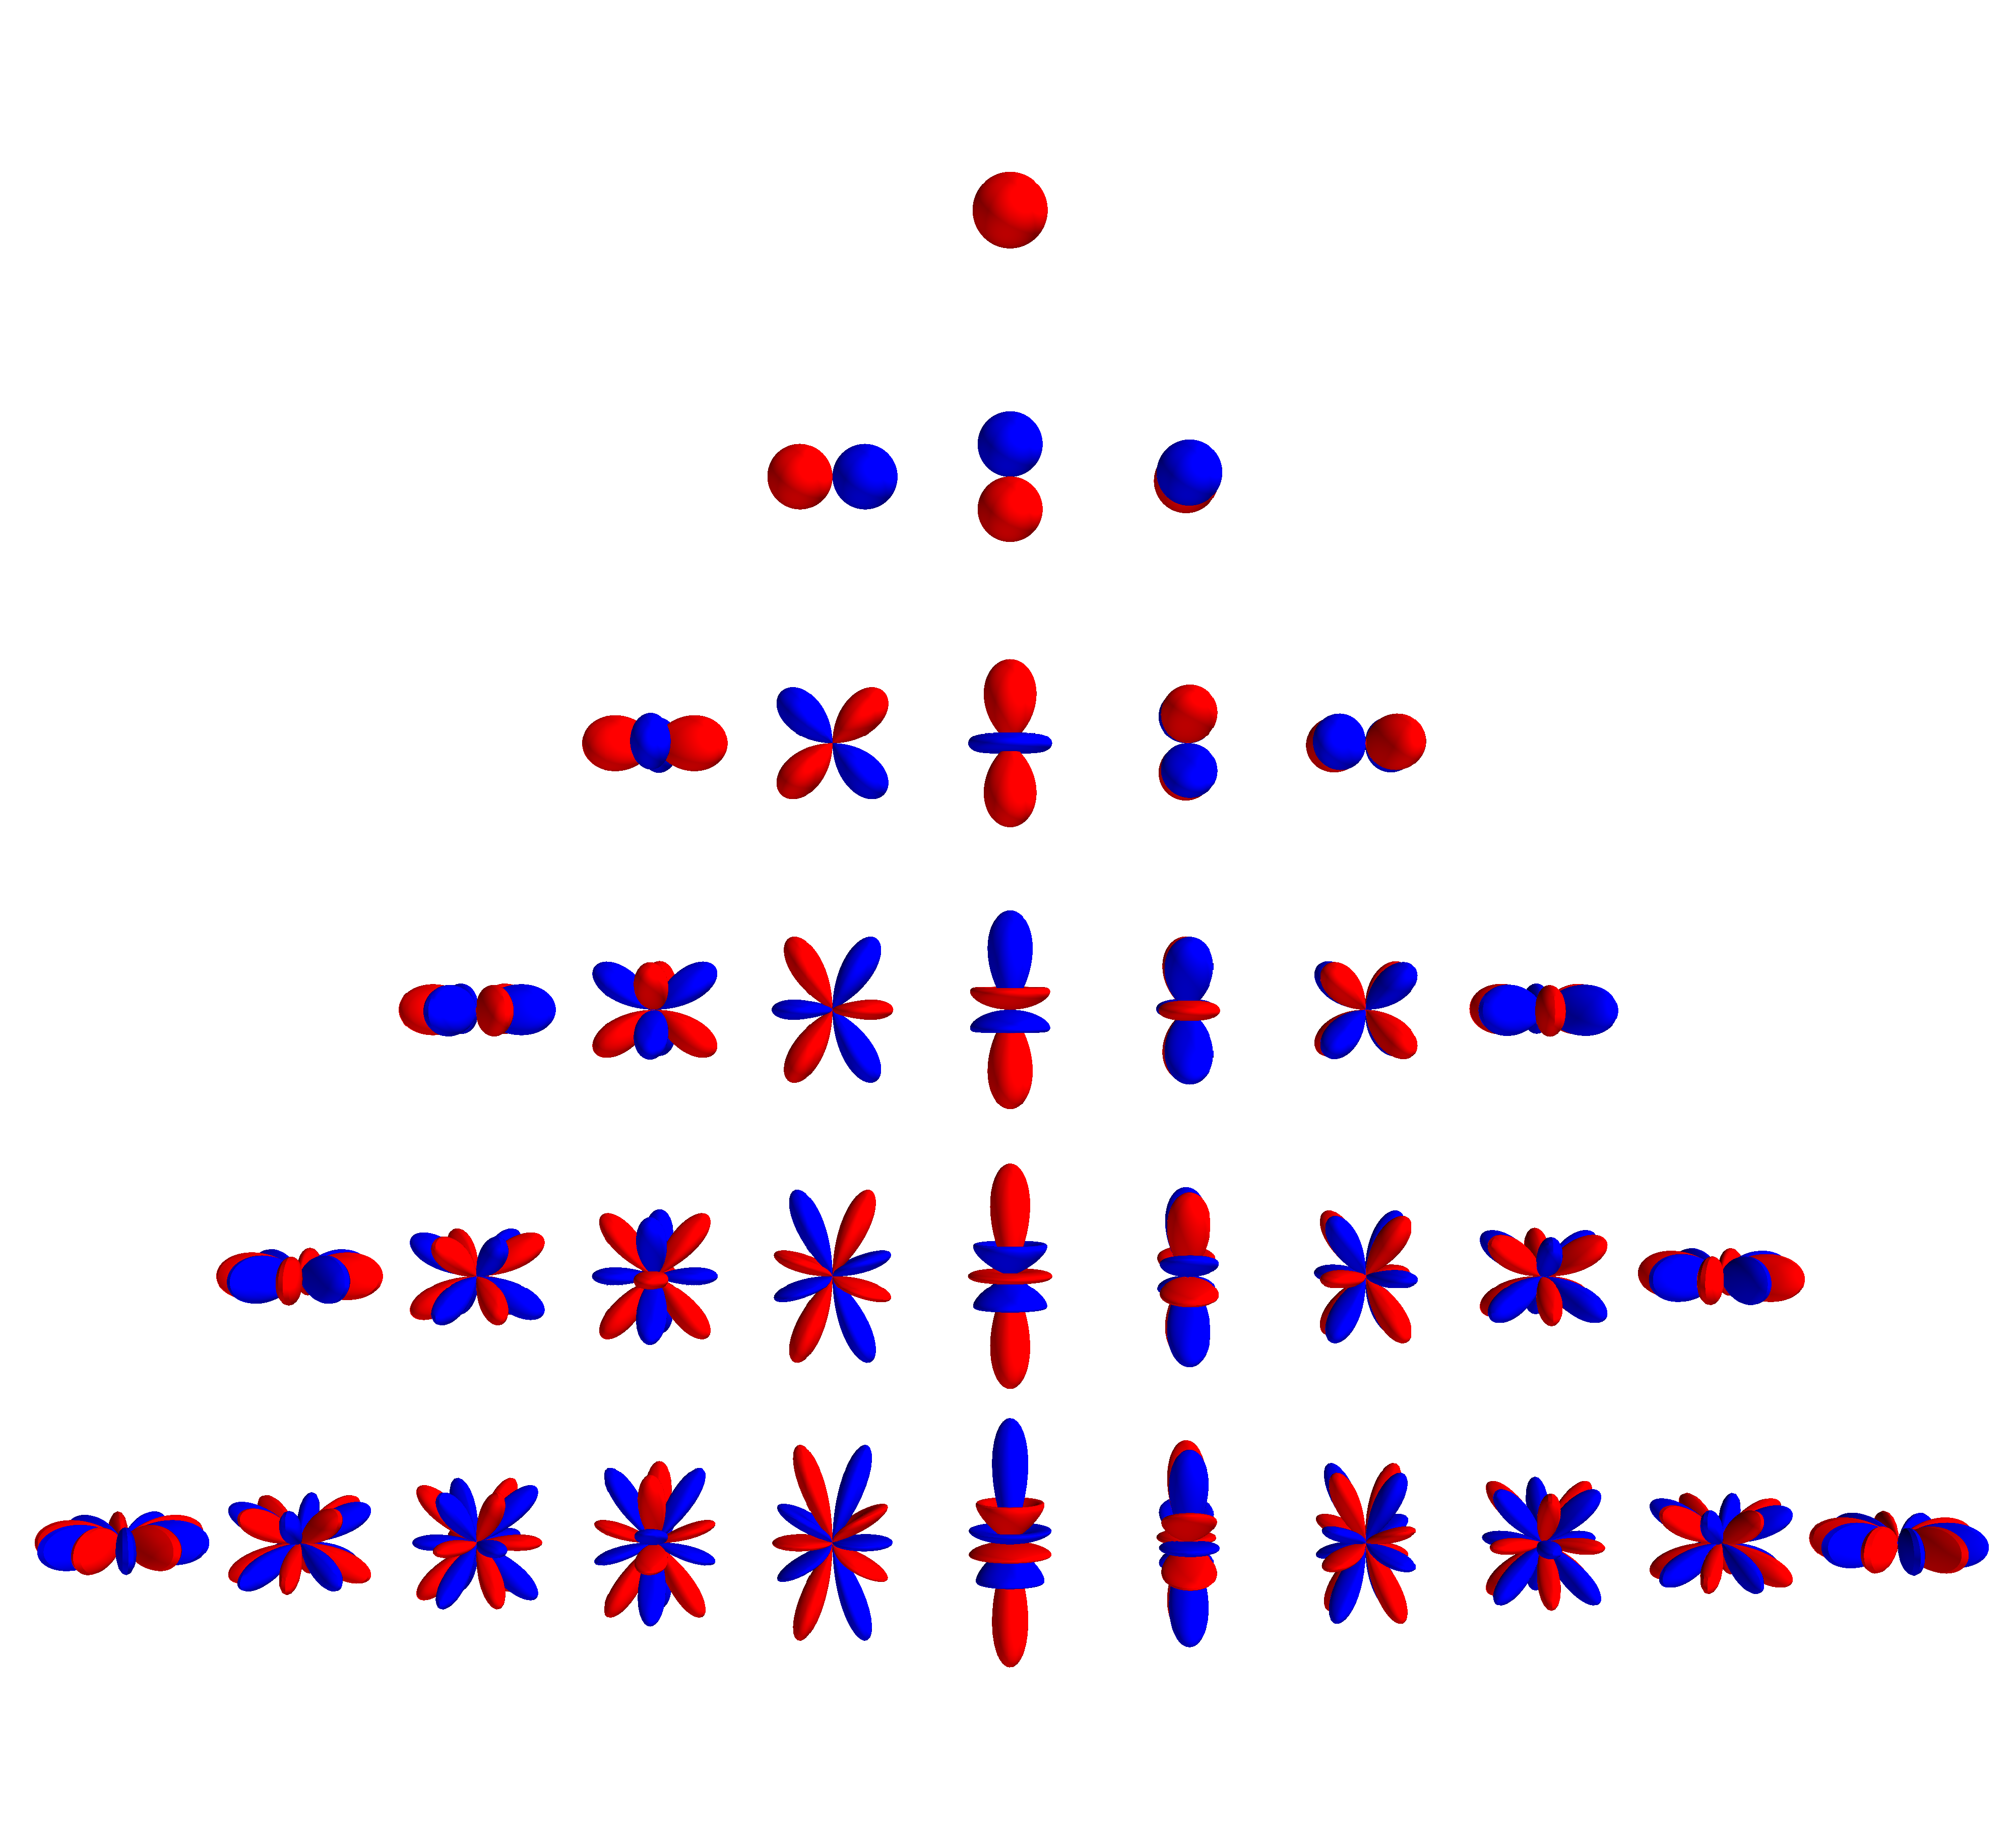
\includegraphics[width=\textwidth, interpolate=true, trim={0em 8em 0em 0em}]{figs/sph_harm}
  \caption{The spherical harmonic functions form an orthonormal basis for functions on the sphere. Red = positive, blue = negative.} 
  \label{fig:test1}
\end{minipage}%
\hspace{0.75em}
\begin{minipage}{.45\textwidth}
  \centering
  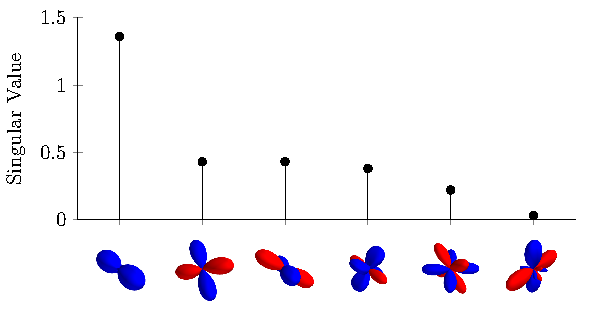
\includegraphics[width=\textwidth, interpolate=true]{figs/svs_dispim}
  \captionof{figure}{The angular singular value spectrum of a polarized
    dual-view selective plane microscope. In the same way that the modulation
    transfer function (MTF) characterizes the ability of an imaging system to
    transfer spatial harmonics, the angular singular value spectrum measures the
    ability of an imaging system to transfer spherical harmonics.}
  \label{fig:test2}
\end{minipage}
\end{figure}

\noindent\textbf{Expected outcome:} A set of software tools that can be used
to reconstruct, visualize, and understand fluorophore orientations from data
collected by a wide class of polarized multiview microscopes.

\noindent\textbf{Potential complications:} We anticipate computationally
expensive reconstructions and visualizations as we refine our pipeline with
increasingly realistic physical models. We plan to employ graphical processing
units (GPUs) and cluster computing to ease the burden.

\noindent\textbf{Aim 2:} Demonstrate and verify three-dimensional fluorescence
orientation microscopy using a dual-view selective plane microscope and a
light-field microscope.

\noindent\textbf{Methods:} To demonstrate the dual-view selective plane
microscope we will use the dual inverted selective-plane illumination
microscope (diSPIM) platform developed by collaborators at the National
Institutes of Health (NIH). Prototype systems are available at the NIH and the
Marine Biological Laboratory (MBL). To demonstrate the light-field microscope we
will use a prototype system that is available at the MBL.

To verify our systems we will use several specimens with a known coupling
between fluorophore position and orientation. We are currently evaluating
several samples for this purpose---PBT
[poly(1,4-phenylene-2,6-benzo-bis-thiazole)] film, giant unilamellar vesicles
\cite{schmid}, and actin networks.

\noindent\textbf{Expected outcomes:} Clear evidence that our microscopes and
reconstruction techniques can reconstruct the position and orientation of
fluorophores in a known sample. 

\noindent\textbf{Potential complications:} We expect initial disagreement
between our results and our known samples due to our use of simplified linear
models. We expect to be able to explain these discrepancies, and we plan to
refine our models if it is computationally feasible.

\noindent\textbf{Aim 3:} Demonstrate the value of three-dimensional fluorescence
  orientation microscopy for live-cell imaging.

\noindent\textbf{Methods:} We will collaborate with biologists at the Marine
Biological Laboratory to find applications for our techniques. We have already
identified several promising areas where the orientation of fluorophores in
three dimensions could report useful information:
\begin{itemize}
\item Cellular migration---the dynamics of actin networks responsible for
  cellular migration have been successfully studied with two-dimensional
  fluorescence orientation microscopy \cite{mehta2016}. We expect that more
  conclusions can be drawn using three-dimensional techniques.
\item Cellular transport---motor protein dynamics have been studied extensively
  using single-molecule techniques \cite{toprak2006}. Our proposed techniques
  may be able to improve on existing measurements.
\item Protein-protein interactions---fluorescence resonance energy transfer
  (FRET) is a widely used technique for measuring nanometer-scale distances
  between proteins. Most FRET experiments make assumptions about the relative
  orientation of the fluorophores involved \cite{nov2006}, and we expect that the
  proposed techniques could address these assumptions and improve the technique.
\end{itemize}

\noindent\textbf{Expected outcomes:} A biological research application for
three-dimensional fluorescence orientation microscopy.

\noindent\textbf{Potential complications:} This aim depends on the previous two
aims, and it requires a collaboration with a to-be-identified biologist. With
our preliminary results in hand, we plan to start searching for a biological
collaborator soon. During the summer the MBL acts as a hub for biologists and
microscopists to test new techniques, so we expect to find a well-defined
biological application in coming months.

\subsection*{Timeline}
\begin{table}[H]
%  \hspace{-1em}
\begin{ganttchart}[%Specs
     y unit title=0.5cm,
     y unit chart=0.5cm,
     vgrid,hgrid,
     title height=1,
     title label font=\bfseries\small,
     bar/.style={fill=gray},
     bar height=0.4,
     group left shift=0,
     group right shift=0,
     group top shift=0.2,
     group height=.4,
     group peaks width={0.1},
     group peaks tip position={0},
     group peaks height={0.1},     
     inline]{1}{24}
    \gantttitle[]{2018}{9}
    \gantttitle[]{2019}{12} 
    \gantttitle[]{2020}{3} \\
    
    \gantttitle{Q2}{3}
    \gantttitle{Q3}{3}
    \gantttitle{Q4}{3}
    \gantttitle{Q1}{3}
    \gantttitle{Q2}{3}
    \gantttitle{Q3}{3} 
    \gantttitle{Q4}{3}
    \gantttitle{Q1}{3}\\

    \ganttgroup[inline=false]{Aim 1: Reconstruction pipeline}{1}{18}\\ 
    \ganttbar[inline=false]{Light-sheet reconstructions}{1}{3}\\
    \ganttbar[inline=false]{Visualization}{1}{6}\\
    \ganttbar[inline=false]{Light-field reconstructions}{4}{9}\\
    \ganttbar[inline=false]{Refine our techniques}{7}{18} \\

    \ganttgroup[inline=false]{Aim 2: Experimental verification}{1}{18} \\
    \ganttbar[inline=false]{Identify test specimens}{1}{3} \\
    \ganttbar[inline=false]{Verify light-sheet microscope}{1}{6} \\
    \ganttbar[inline=false]{Verify light-field microscope}{4}{9} \\
    \ganttbar[inline=false]{Verify refinements}{7}{18} \\

    \ganttgroup[inline=false]{Aim 3: Live-cell demonstration}{4}{21} \\ 
    \ganttbar[inline=false]{Identify research question}{4}{12} \\
    \ganttbar[inline=false]{Investigate research question}{10}{21} \\
    \ganttbar[inline=false]{\textbf{Thesis}}{22}{24}
  \end{ganttchart}
  \caption{Proposed project timeline.}
  \end{table}

\section*{References}
\setlength\biblabelsep{0.01\textwidth}
\printbibliography[heading=none]

\end{document}